% Created 2022-10-02 Sun 13:48
% Intended LaTeX compiler: pdflatex
\documentclass[11pt]{article}
\usepackage[utf8]{inputenc}
\usepackage[T1]{fontenc}
\usepackage{graphicx}
\usepackage{grffile}
\usepackage{longtable}
\usepackage{rotating}
\usepackage[normalem]{ulem}
\usepackage{amsmath}
\usepackage{textcomp}
\usepackage{amssymb}
\author{Alejandro Hervella, Peter Brown, Ian Chan, Gokce Saracoglu, Will Tower}
\date{\today}
\title{Capstone 1 Weekly Report}
\begin{document}

\maketitle
\tableofcontents


\section{Summary of Accomplishments}
\label{sec:orgf4c217c}

Several discussions pertaining to project viability:

\section{Capstone adviser meeting}
\label{sec:org0e64d2a}
The team met with Masoud in the ECE capstone lab to discuss project proposals, expectations, and what effort results in a succesful team. Ten ideas were briefly discussed:

\begin{enumerate}
\item Airdrop phone case
\begin{itemize}
\item Nixxed on grounds of low complexity
\end{itemize}
\item Remote Light switch
\begin{itemize}
\item Proposal involved a set of light modules connected and controlled by an IoT protocol, nixxed on grounds of low complexity.
\end{itemize}
\item Portable arcade cabinet–Alejandro
\begin{itemize}
\item Proposal involved af portable arcade cabinet/console platform with several modular components designed to provide AR experiences to end users.
\end{itemize}
\item Parallel Robotics–Will
\begin{itemize}
\item Proposal involved design of a cable driven parallel robot, a generic device with broad applications in warehousing, manufacturing, pick-and-place, biological testing, and automation.
\end{itemize}
\item Garbage-Robotics Assist–Ian
\begin{itemize}
\item Proposal involved design of a 'catcher robot,' with a drive chassis and optical sensor. Team conceived the robot as tracking parabaloids in space using machine vision, and centering itsself under them.
\end{itemize}
\item wheelchair that sends sms if ekg signals goes out (wheelchair)--Gogo
\begin{itemize}
\item Proposal involved a wheelchair with several integrated biomedical sensors designed to alert relevant caretakers of problems.
\end{itemize}
\item Active control for a wheelchair that stays upright
\begin{itemize}
\item Proposal involved design of a wheelchair which operates as an inverted pendulum (similar to a Segway). User would control device with abdominal movements. Target market: those with need of a wheelchair and a desire to prevent acute muscular atrophy.
\end{itemize}
\item Muscle sensors to see what needs working or is chronic (for elderly)(cardio and muscle activity tracker)
\begin{itemize}
\item Proposal involved a number of biomedical sensors used to create a heatmap of individual muscular states.
\end{itemize}
\item E-Ink Keyboard–Peter
\begin{itemize}
\item Proposal involved creation of a keyboard device with paper-white e-ink keycaps, allowing users to switch alphabets and layouts while maintaining an accurate visualization. Proposed market is multilinguals, superusers with dynamic keybinding needs, and DVORAK afficianados.
\end{itemize}
\end{enumerate}

\section{Breakout Meeting + Defense in the Radio Lab}
\label{sec:org2c82291}
\textit{<2022-07-18 Mon 16:00>--<2022-07-18 Mon 19:00>}

Projects in the above section tagged [ -- NAME ] were selected as roughly viable, and the team decided to move forward with more formal defenses. Gokce was unable to attend due to a medical emergency.

\subsection{E-Ink Keyboard}
\label{sec:org623a5c6}

By adding e-ink displays into the keycaps, we can dynamically set the value of the key and display the value on each keycap.  This will allow users who require multiple keyboard layouts to switch quickly and easily, and will no longer be required to memorize multiple layouts.

The value of e-ink displays is the low energy requirements for the screen and the screens do not require continuous power to display text, unlike LCD screens.

\subsubsection{Market: There are two large groups of users that this keyboard would be designed for:}
\label{sec:orgdfdf823}

Bilingual/Polyglot writers : For any customer that regularly types in multiple languages, they often have to rely on brute memorization if they are working on a language that does not have the default QWERTY layout.  For these users, they will be able to switch between these two layouts quickly and easily, and the screens on each keycap will reflect the configuration that the user selects. 

Software power users : Users of applications such as Photoshop, After Effects, and AutoCAD make extensive use of keyboard shortcuts to accelerate their workflow.  For these segments of users, having a keyboard that can reflect the shortcuts on the keyboard itself will be valuable, as it will let users store multiple configurations without requiring to commit all of them to memory.

\subsubsection{How It might be built :}
\label{sec:org616499c}
The EIK would be constructed similarly to a regular keyboard, complete with a case, and key switches. There would be three custom components to design, for example a custom pcb to handle the displays associated with each keycap.  In addition, custom plastic coverings would need to be manufactured to account for the circuitry involved with the screens.
    The keyboard pcb would consist of a keyboard matrix,a circuit lattix of M x N junctions, with each one a keycap.  Pressing the key would complete a circuit, which reading the position would allow us to determine which key was pressed.  Using this, we simply pass it into an array and fetch what key it is mapped to, and send that to the computer.

\subsubsection{Positives of developing:}
\label{sec:org4473c3f}
Prior art : Thankfully, there is ample material to create keyboards, such as KiCAD libraries for footprints of keyboard components
Solves an actual issue: The ability to display different keys without physically switching them is a boon for both bilingual users, as well as power users who use their keyboard extensively for software they use.
Modular complexity : Being able to construct different types of keyboards, as well as a plethora of premade components, means that this keyboard can be as complex or as simple as required.
Foreseeable problems
\subsubsection{Cost :}
\label{sec:org1daecf3}
E-ink displays are prohibitively expensive, with preliminary searches costing \$\textasciitilde{}5.80 per display. At the smallest possible keyboard size (50\%), there are a minimum of 60 keys, bring the cost to \textasciitilde{}350 dollars, which is nearly half the budget.
\subsubsection{Lead times:}
\label{sec:orge00c825}
There are very few e-ink manufacturers, and even less so at the sizes that we would like to purchase
\subsubsection{Impossible to source:}
\label{sec:orgd0ad300}
They don’t make them this size. Seriously.  Smallest ones I could find were 0.96”.  However, I found a suitable replacement here: \url{https://uk.farnell.com/midas/mcot048064a1v-wi/display-oled-graphic-tab-48x64/dp/2817906}.  Only difference is that it’s OLED and 3mm larger than a standard keycap.

\subsubsection{Potential Parts List:}
\label{sec:org8546c70}
\begin{center}
\begin{tabular}{llrlr}
Name & Link & Price & Lead Time & Current Stock\\
I2C OLED Display & \url{https://www.dfrobot.com/product-1353.html} & 15.001 & N/A & 3\\
OLED Display & \url{https://www.mouser.com/ProductDetail/Futaba/ELF1101AA?qs=PqoDHHvF649YYSRiFKJOkQ\%3D\%3D} & 28.00 & 30 weeks & 33\\
Square OLED display & \url{https://www.mouser.com/ProductDetail/Display-Visions/EA-W064048-XALG?qs=f9yNj16SXrJs20LfEzPXZQ\%3D\%3D} & 16.87 & 6 weeks & 5\\
Kailh Choc Red Switch - Low Profile - Linear - 10 pack & \url{https://mechanicalkeyboards.com/shop/index.php?l=product\_detail\&p=6337} & 8.50 (10 pack) & N/A & Enough\\
\end{tabular}
\end{center}


\subsection{Parallel Robotics Application}
\label{sec:orge1f5296}
\subsubsection{Applications}
\label{sec:org94d6c39}

\begin{enumerate}
\item Why would you even want to do this?
\label{sec:orgb4944b9}

\begin{itemize}
\item Two classes of robots
\end{itemize}

\begin{enumerate}
\item serial (like an arm)
\label{sec:org2873d88}

\begin{itemize}
\item positioning error is cumumlative
\item long, complex chain structures
\item rigidity decreases as chain count increases
\item joint flexibility dependent on upstream and downstream joints
\end{itemize}

\item parallel (like a spider)
\label{sec:orgad00264}

\begin{itemize}
\item each chain relatively short and simple in structure
\item resists unnecessary movement
\item chain positioning error is average
\item off-axis flexibility of joints also affected by other chains
\item provides closed-loop stiffness, robot is rigid relative to components
\item rigidity increases as chain count increases
\end{itemize}
\end{enumerate}

\item Who even does this?
\label{sec:org2b58de4}

Anyone who needs really high precision, has comparably small manipulated objects, and is okay with one location


\begin{enumerate}
\item Warehousing
\label{sec:org807d9c1}

\href{https://www.youtube.com/watch?v=2b4YwFZhtIE}{CoGiRo}

\begin{center}
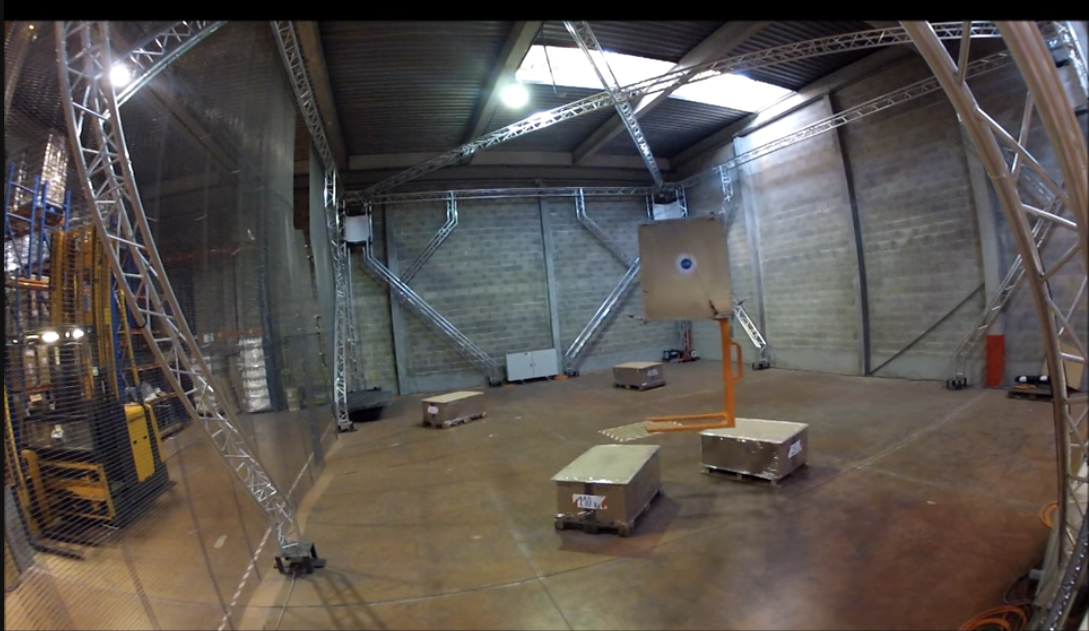
\includegraphics[width=.9\linewidth]{Applications/2022-07-18_12-43-16_screenshot.png}
\end{center}

\item Pick + Place + small object manip
\label{sec:org7b196ec}

Easier + More precise control important/cheaper for small items

\href{https://www.youtube.com/watch?v=QFZMhsVn\_CE}{Pick and Place (China)}

\begin{center}
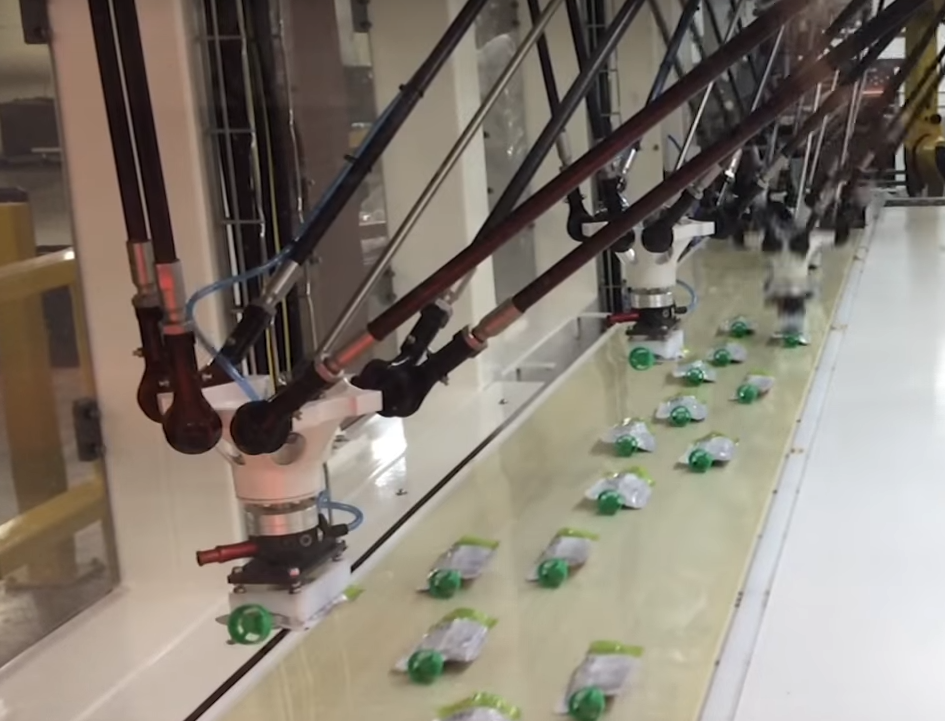
\includegraphics[width=.9\linewidth]{Applications/2022-07-18_12-59-12_screenshot.png}
\end{center}

\item Motion simulator people
\label{sec:orgc69fc1f}

Easier to calculate a specific path in parallel kinematics

\href{https://www.youtube.com/watch?v=9KMptw7ZgVI\&t=1s}{Movin a dude}

\begin{center}
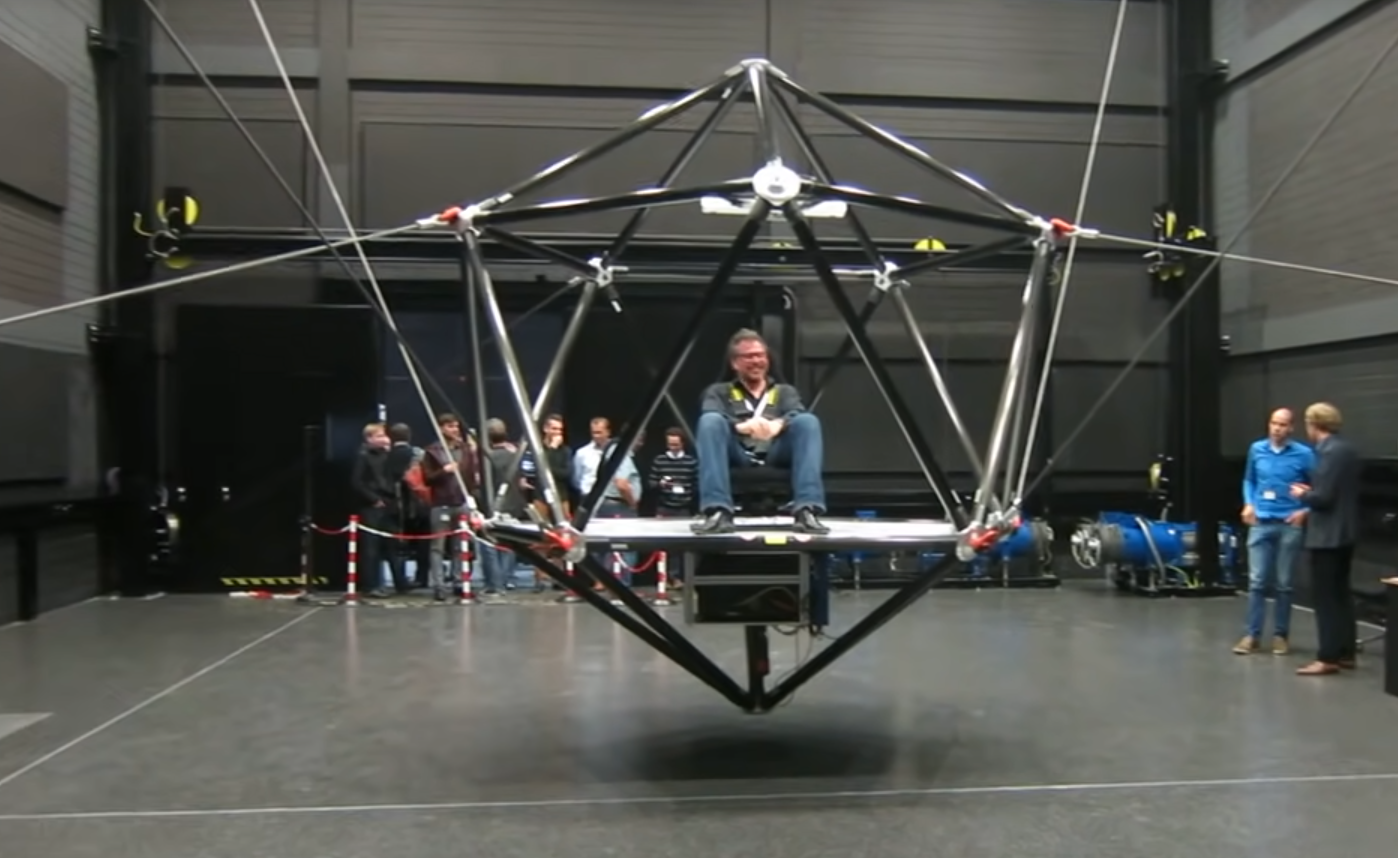
\includegraphics[width=.9\linewidth]{Applications/2022-07-18_13-03-17_screenshot.png}
\end{center}

\item Biomedical people
\label{sec:orge99f0cd}

Just trust me on this one, assaying, test verification, DNA sequencing, all automatable with parallel robotics. Bio people tend not to call it robotics though.
\end{enumerate}
\end{enumerate}

\subsubsection{Mechanical Modules}
\label{sec:org93a5323}

\begin{enumerate}
\item Frame (8020)
\label{sec:org25ffe36}

\href{https://8020.net/20-2020.html}{site}, \$0.25/inch


\item an object
\label{sec:org6717900}
\begin{center}
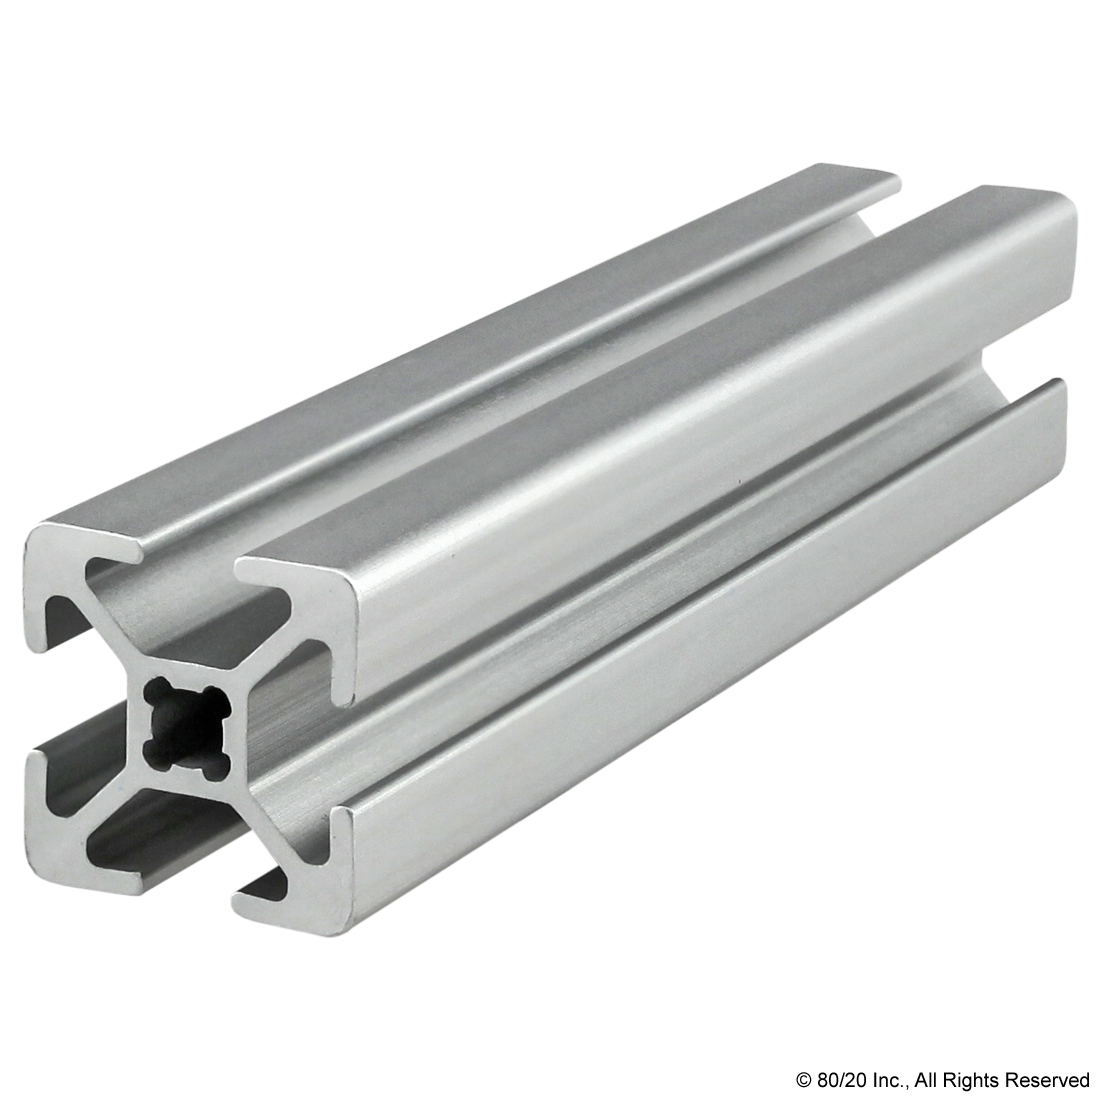
\includegraphics[width=.9\linewidth]{Hardware_needed/2022-07-18_13-11-55_screenshot.png}
\end{center}
\item an assembly
\label{sec:orgd042e0c}
\begin{center}
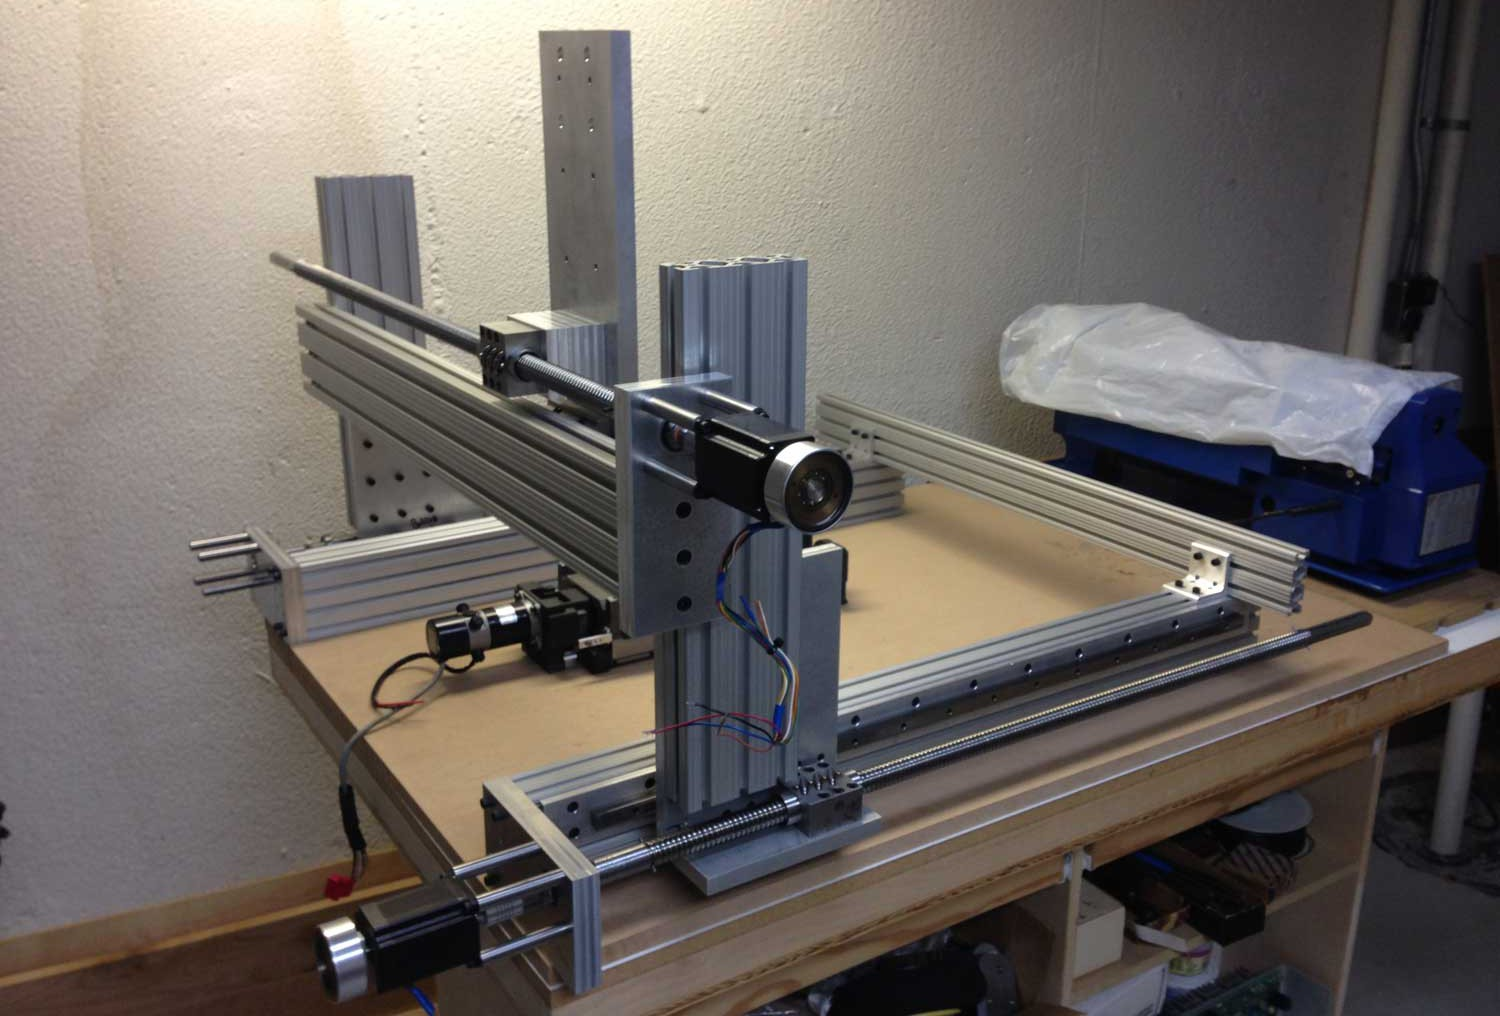
\includegraphics[width=.9\linewidth]{Hardware_needed/2022-07-18_13-13-15_screenshot.png}
\end{center}

\item Effector
\label{sec:org28c9cbf}

Popular to 3d print these for passive end manipulator, probably looking at small sheetmetal project for active manipulator

\item CoGiRo (passive)
\label{sec:org2366bcc}
\begin{center}
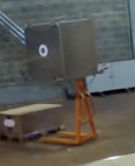
\includegraphics[width=.9\linewidth]{Hardware_needed/2022-07-18_13-31-45_screenshot.png}
\end{center}

\item Winches + Pulleys (they rotate)
\label{sec:org8e74d23}

\begin{center}
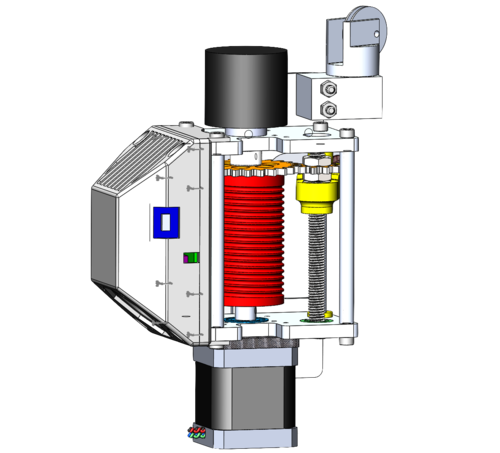
\includegraphics[width=.9\linewidth]{Hardware_needed/2022-07-18_13-16-45_screenshot.png}
\end{center}

\begin{itemize}
\item Probably looks something like that
\begin{itemize}
\item stepper motor (bottom)
\item gearing + screw (right)
\item optical encoder + PCBA for closed loop control (left)
\item pulley (top)
\item this is the mechanically challenging bit
\end{itemize}
\end{itemize}

\item Stepper Motors
\label{sec:orge0ea1b9}

\href{https://www.digikey.com/en/products/compare?s=N4IgzCBcDaIEwBYCMB2ADHArCANCBAHAmAlriJgJyWZoqXkBsmBBmKKIAunglCAHoApgDsBABwBOAewAmAVwDGAFwDOAgGYBLADbKhkgav3jxBgLQBbacumT1qSgH5VAXgByCAJIBzAFYAwgBCitIAogAeSNIAIgDiAKpBlkExAILuPgBaAO4A0gCaQdIAikEoeWkARgBKQT4AEgVFlmFplmkAaj5pWQCGAWkA8gCyGX7iAdLiBNKKJWkAGiVeaQ1pAZglC1klANZpImkAUgVpKMMFPQBuPgAqaUFD7n6lABZ7e7LuIhEAYgBlLzHLR5NA9ZQxMIABTify6YGhfy8WSCflk11k0i8NQWdz6d1UOWOPjeETyCR8JQaPgOdwAXmFFASSqosmk0O5ViAAL5AA}{comparison on digikey}

Tricky to buy these guys, they tend to be expensive per unit on Digikey and I'd need to do \textasciitilde{}1 day of research into the minimum viable motor

\item Mounts
\label{sec:org240b1cc}

Mounting on 8020 is super easy, literally like legos
\end{enumerate}

\subsubsection{Electronics Modules}
\label{sec:org1b61546}

\begin{enumerate}
\item Effector Controller
\label{sec:orgfa1fe99}

\begin{itemize}
\item small PCBA for actuating whatever is on the effector
\item communication is possible by a trailing cable assembly or wireless
\begin{itemize}
\item cable for something requiring significant power
\item wireless for low power application
\end{itemize}
\end{itemize}

\item Generic Rotary Encoder
\label{sec:org8863021}

\begin{itemize}
\item You can buy these on Digikey
\item usually easy to interface them with your custom hardware (SPI/CAN/etc)
\end{itemize}

\begin{center}
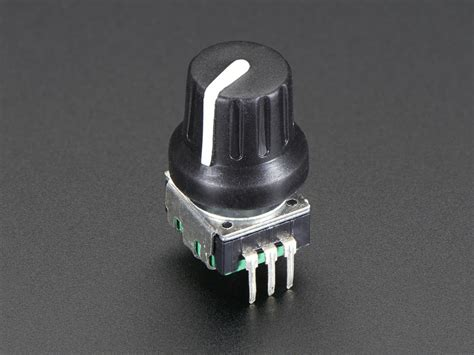
\includegraphics[width=.9\linewidth]{Electronics_Modules/2022-07-18_13-48-01_screenshot.png}
\end{center}

\item Generic Stepper Motor Driver
\label{sec:org2cf24f3}

\begin{itemize}
\item You can buy these on Digikey
\item Piece of hardware that generates and sends signals to our selected stepper motor
\end{itemize}

\item Main Control Board
\label{sec:orgf501a3a}
handles:
\begin{itemize}
\item pathing and kinematics
\item calibration (likely by limit switch?)
\item rotary encoder info streams
\item connection to effector
\item any fancy active controls we want to implement (like robotic vision)
\end{itemize}
probably needs to be specced for running some ROS modules, MSP432 dev boards run \$50/piece, beaglebone black SBC, or EMC32 line are also good choices
\begin{center}
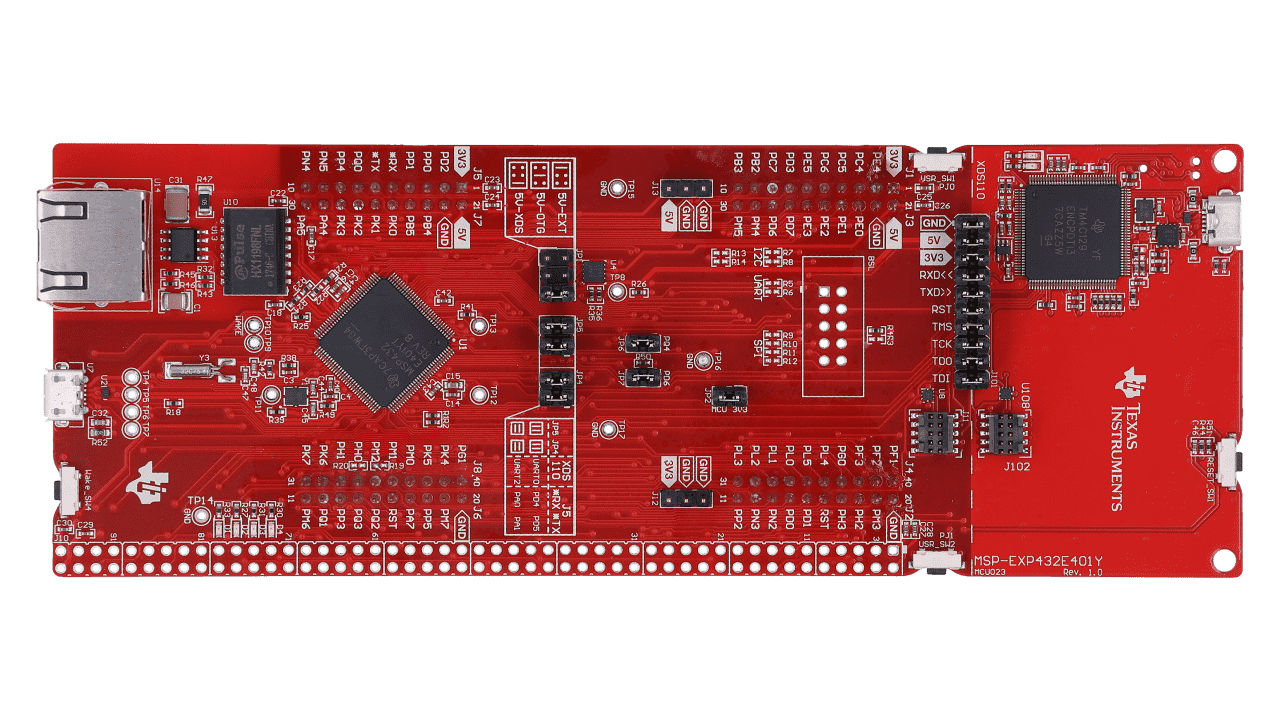
\includegraphics[width=.9\linewidth]{Main_Control_Board/2022-07-18_14-30-59_screenshot.png}
\end{center}
\begin{center}
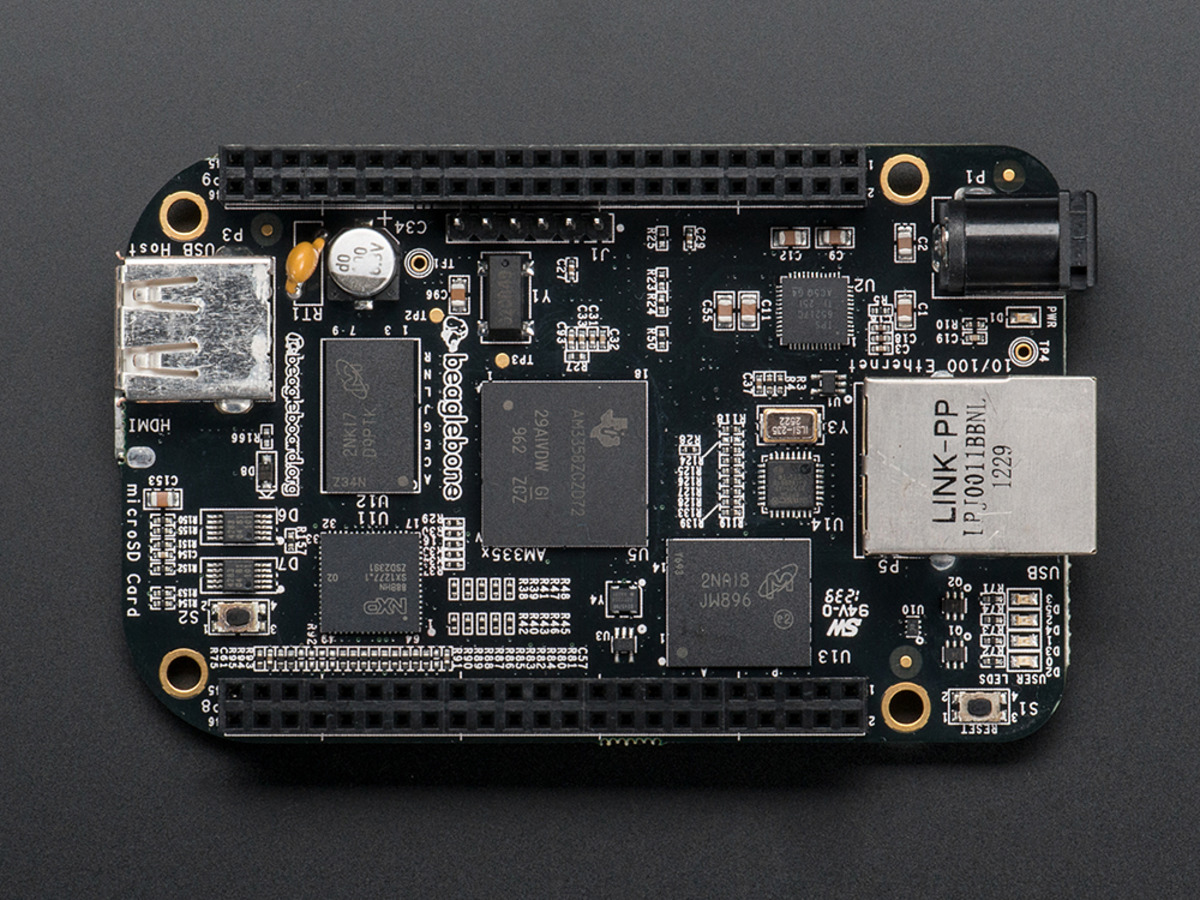
\includegraphics[width=.9\linewidth]{Main_Control_Board/2022-07-18_14-28-49_screenshot.png}
\end{center}

\item Power Supply Unit
\label{sec:org0b31321}
\begin{center}
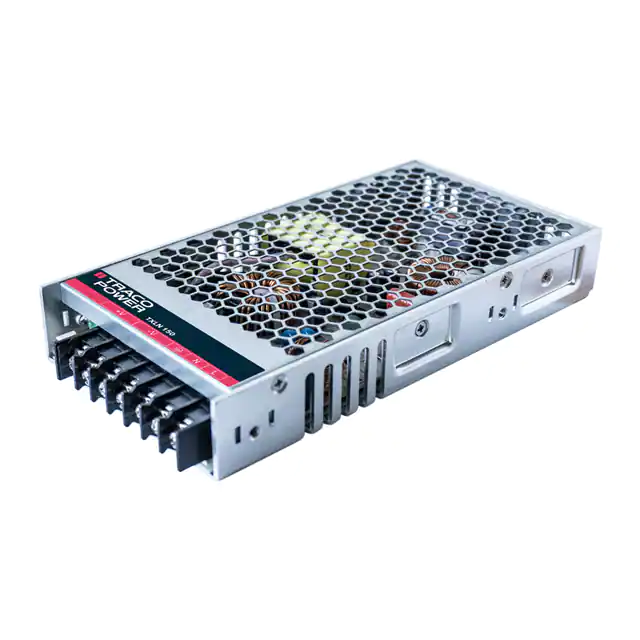
\includegraphics[width=.9\linewidth]{Power_Supply_Unit/2022-07-18_14-27-16_screenshot.png}
\end{center}
Hard to size until you know what stepper motors are drawing, what your central board is specced for, if you want to do any advanced + special control gizmos. Fermi estimate says
\begin{itemize}
\item 16 W for main board (based on beaglebone SBC max draw
\item Extremely liberal 12 W / Stepper Motor
\item Give +40\% for margin
\end{itemize}
\begin{verbatim}
SBC = 16;
SM = 12*8;
MARGIN = 1.4;
fermi_total = MARGIN * (SBC + SM)
\end{verbatim}
Tends to run \textasciitilde{}\$75/unit on Digikey, \href{https://www.digikey.com/en/products/detail/traco-power/TXLN-150-124/13681763}{link}
\end{enumerate}

\subsubsection{Some Decent Whitepapers}
\label{sec:orgc274b9f}

\href{https://www.cambridge.org/core/services/aop-cambridge-core/content/view/B129C939BF4491AA693A36A54AE6D2C7/S0263574721001971a.pdf/full-dynamic-model-of-3-upu-translational-parallel-manipulator-for-model-based-control-schemes.pdf}{Kinematics for parallel control schemes}
\href{https://ieeexplore.ieee.org/stamp/stamp.jsp?arnumber=9737194}{on dealing with tension in large cable-driven systems}
\href{https://ieeexplore.ieee.org/stamp/stamp.jsp?arnumber=9737158}{dynamic calibration of cable-driven systems}
\href{https://arxiv.org/pdf/2003.08860.pdf}{adaptive control under uncertainty in parallel robotics}

\subsubsection{Challenges}
\label{sec:orgec4890b}

\begin{itemize}
\item Custom hardware at microcontroller level can be tricky
\item Winch design likely to involve some interaction with mechanical engineering
\item Real time kinematics calculations can be a challenging CS thing, getting to the correct O(n) is critical
\item Active position control can be mathematically involved sometimes
\item Robotics can be mathematically involved sometimes
\item Cable tension problems must be accounted for; for high speed or high robot:object mass ratios
\end{itemize}

\subsubsection{Vision Applications}
\label{sec:org794f5da}

If we feel ambitious the clear thing to do in robotics is usually to add a camera + vision daughter board, demonstrate that we can throw and catch items. I have not done vision like this, super speculative.


\subsection{Trash Bot}
\label{sec:org2dfda01}

Original Ideas
1 - Trash can that detects the trajectory of the flying trash and moves to catch it
2 - Trash can with multiple “plates” on the edge of the lid that can lift and block the flying trash to prevent missing
**idea 2 sounds easier to do than 1, but idea 1 is more interesting and has a higher success rate because it isn’t stationary (allows a wider range to “catch”)

Pros:
\begin{itemize}
\item throws is appealing
\item being thrown out (office (paper), warehouse (cardboard), etc.)
\end{itemize}

Cons:
\begin{itemize}
\item Powering trash bin can introduce sustainability problem
\item Unnecessary robot to have in most cases (placing waste bin next to you)
\item Limited in size
\item Isn’t the most ground breaking idea
\end{itemize}









\subsection{Wheelchair Alert System}
\label{sec:orgb798d46}

\subsubsection{Synopsis}
\label{sec:org3a033d8}
Wheelchair safety has remained a strong innovation topic in the healthcare industry as the number of wheelchair users grows at a rapid rate. In 2016, there were over 3.3 million wheelchair users in the United States alone with 1.825 million of those users aged 65 or above. With this strong number of elderly wheelchair users, the probability of wheelchair prone injuries increases. Out of all wheelchair injuries, wheelchair tips and falls lead as one of the highest cases as a study in 2003 found that tips and falls accounted for approximately 65-80\% of all wheelchair related injuries. Additionally, as increased innovation is made towards furthering wheelchair user independence in society, the likelihood of wheelchair users living alone is expected to rise. There is a robust financial case to make our wheelchair safety system a viable business. There are no intelligent wheelchair systems available, despite the large market. Senior citizens with limited mobility are also often unable to live autonomously. Living under constant care in a nursing home or a relative while performing simple chores becomes difficult. Currently, no solution alerts caregivers and close contacts when an individual who uses a wheelchair tips and falls. The market has a few similar ideas, but there have been none that have exited the design phase.

\subsubsection{Pros and Description}
\label{sec:org0444fa9}
This project will be focused on developing a smart wheelchair system capable of reading both wheelchair motion and user heart rate in real-time to detect when wheelchair falls have occurred. Using the live data, an alert is immediately sent to caretakers or loved ones through SMS or an app alert when a wheelchair fall has been detected, allowing for prompt and possibly life-saving care for the wheelchair user. Based on this main hypothesis, the following objectives for this project are formulated: a.) to detect when a wheelchair/user falls in either left, right, forward, or backward direction; b.) monitor heart rate of user; c.) provide immediate communication of fall to caretaker/loved one. Potentially an app could be created to keep all the heart rate data recorded for future use and a notification would be sent to the caretakers or loved ones in case of a fall. The goal of our heart rate monitoring objective is to provide caretakers and doctors with more patient data to allow for a thorough analysis post-fall of a patient’s medical health. This feature is also especially beneficial for those with heart disease and special reduced mobility.

\subsubsection{Cons}
\label{sec:org0767d41}
The biggest issue with this project would be novelty as our professor mentioned. There were many projects made in the previous semesters using a wheelchair which could potentially make this idea rather “simple”. We might need to add more features to make it more complex (eg. Active control to stay upright, airbags etc). Signal processing for the ECG data might take longer to perfect by trial and error, that might be why it might be better to analyze ECG data on MATLAB before writing code in another language.

For this design, we can use the 3-Axis ADXL335 Accelerometer which costs between \$14.95-16.50 and connect it to an Arduino. For the ECG component we can either use the SparkFun Single Lead Heart Rate Monitor AD8232 (\$21.50) or build the ECG on a breadboard using low pass and high pass filters and an amplifier and connect it to an Arduino. Building an ECG on a breadboard will cost around \$100.

The design will first start the calibration by connecting to the Arduino board and start data acquisition for a few seconds to calculate the threshold and alert levels. After the calibration is completed live data tracking with alerts will be enabled and the program will check for breaches of alert levels. When the collected data Is above or below a certain threshold, alerts will be triggered, and a notification is sent.

\subsubsection{Paths to Market}
\label{sec:orgd07b39b}
There are numerous paths to market for this design; these include selling the intelligent wheelchair safety system directly to the patients and their families, selling to hospitals, and selling to assisted living homes. The unique selling proposition for this product is its intelligence - by automatically detecting and reporting a tip or fall to the user’s close contact and healthcare provider, pertinent data is relayed almost immediately, and the user can receive assistance faster. These scenarios often occur when the user is too injured or disoriented to contact their loved ones for help. The healthcare provider can also stream ECG data from the time of the accident to view heart rate information, adding additional information that may be pertinent when assisting an individual. After reading numerous case studies and reports, an appropriate business model is identified, which considers a gap in the market, addressed via this innovative solution.

\subsubsection{Increasing Complexity}
\label{sec:org794ab4a}
\begin{itemize}
\item Active control for a wheelchair to stay upright (would not need fall detection)
\item A device to help stand up from a wheelchair
\item EMG sensors to measure muscle response (could be useful for users who have limited muscle activity to see the response to the nerve’s stimulation of the muscle)
\end{itemize}


\subsubsection{Related research on smart wheelchairs}
\label{sec:orgee6eb4b}
H. Vora, A. Gupta, C. Pamnani, and T. Jaiswal, “Multimodal Smart wheelchair integrated with safety alert system,” International Journal of Engineering and Advanced Technology, vol. 9, no. 4, pp. 1324–1330, 2020.

M. A. Rahman, S. M. Ahsanuzzaman, A. Hasan, I. Rahman, T. Ahmed and M. M. Kadir, "Building A Wheelchair Controlling and Fall Detection System Using Mobile Application," 2020 2nd International Conference on Advanced Information and Communication Technology (ICAICT), 2020, pp. 213-218, doi: 10.1109/ICAICT51780.2020.9333478

\section{Breakout Meeting on Zoom}
\label{sec:org318b56f}
\textit{<2022-07-19 Tue 17:00>--<2022-07-19 Tue 18:30>}
Further refinement and discussion of ideas, Will was unable to attend due to a personal matter.
\end{document}